\section{Análise de métodos de atribuição de estrutura secundária}

Diferentemente de vários métodos publicados de predição de estrutura secundária que utilizaram os resultados de atribuição provenientes de apenas um método, comumente o DSSP, nós optamos por utilizar os resultados de um consenso entre quatro métodos. Consequentemente, é importante analisar como esses métodos diferem entre si.

As diferenças entre as metologias de atribuição foram previamente discutidas na seção \ref{section:metodos_atribuicao}. Nesta seção, analisaremos as diferenças nas estruturas secundárias atribuídas aos resíduos.

As análises a seguir foram feitas entre os resíduos de 6749 proteínas do banco de dados Top8000-HOM50 que tiveram estrutura secundária atribuída por todos os métodos. Isso excluí 5,19\% dos resíduos que não tiveram a estrutura secundária atribuída por não terem sido visualizados na estrutura experimental e 0,05\% dos resíduos que não tiveram sua estrutura atribuída por um ou mais programas devido à possíveis falhas dos programas. 

Notamos que, entre os quatro métodos de atribuição analisados, há a ocorrência de uma variação considerável entre as estruturas secundárias atribuídas para cada resíduo. A figura \ref{fig:comparacao_metodos_atribuicao} demonstra a similaridade observada entre os métodos. Como esperado, a maior similaridade é observada entre os métodos DSSP e STRIDE, uma vez que o último é inspirado no primeiro. Entretanto, a similaridade entre os demais métodos encontra-se na faixa entre 83\% e 85\%. A porcentagem de resíduos que apresentaram consenso entre os quatro métodos foi de apenas 74,43\%.








\begin{figure}
  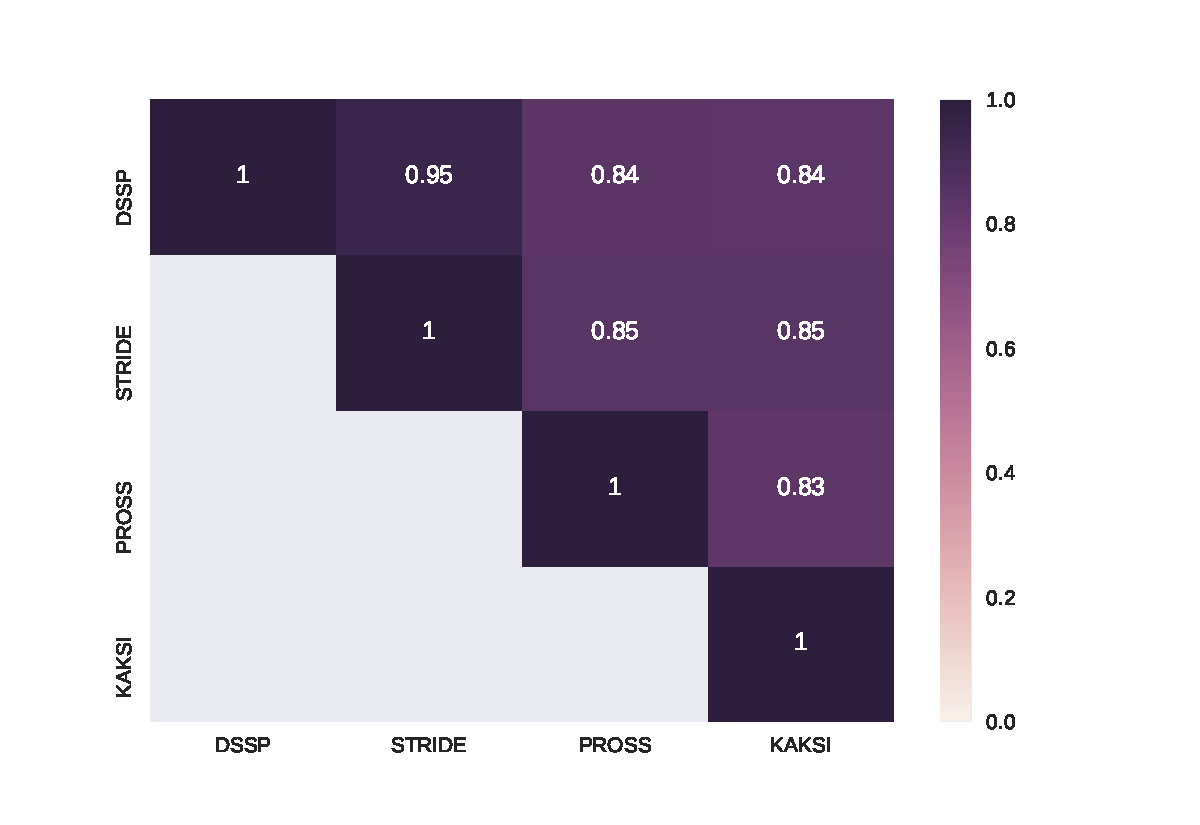
\includegraphics[width=\linewidth]{../figures/comparacao_metodos_atribuicao.pdf}
  \caption{Similaridade entre as estruturas secundárias atribuídas para cada resíduo entre os quatro métodos de atribuição de estruturas secundárias: DSSP, STRIDE, KAKSI e PROSS.}
  \label{fig:comparacao_metodos_atribuicao}
\end{figure}


\begin{figure}
  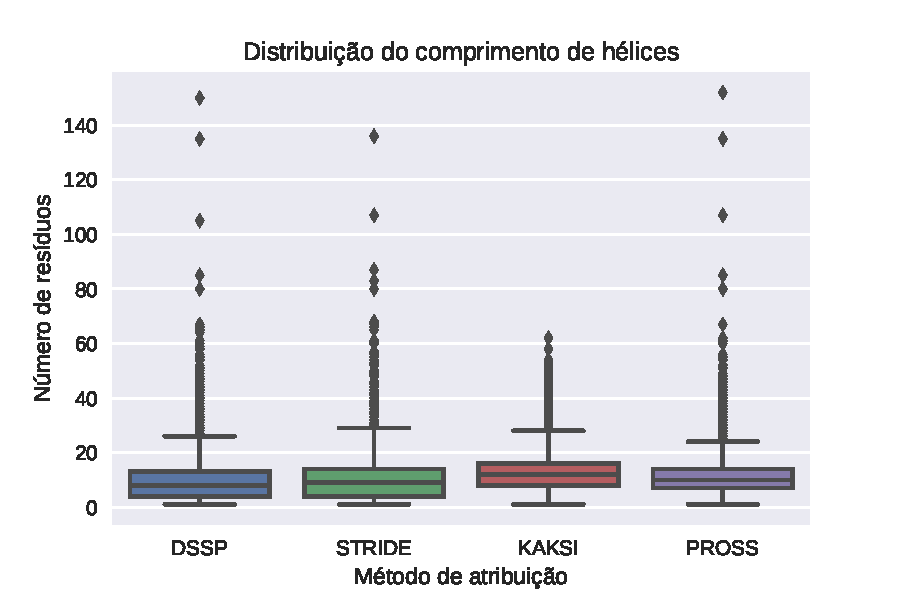
\includegraphics[width=\linewidth]{../figures/distribuicao_comprimento_helices.pdf}
  \caption{Distribuição do comprimento de hélices por método de atribuição de estrutura secundária.}
  \label{fig:distribuicao_comprimento_helices}
\end{figure}

\begin{figure}
  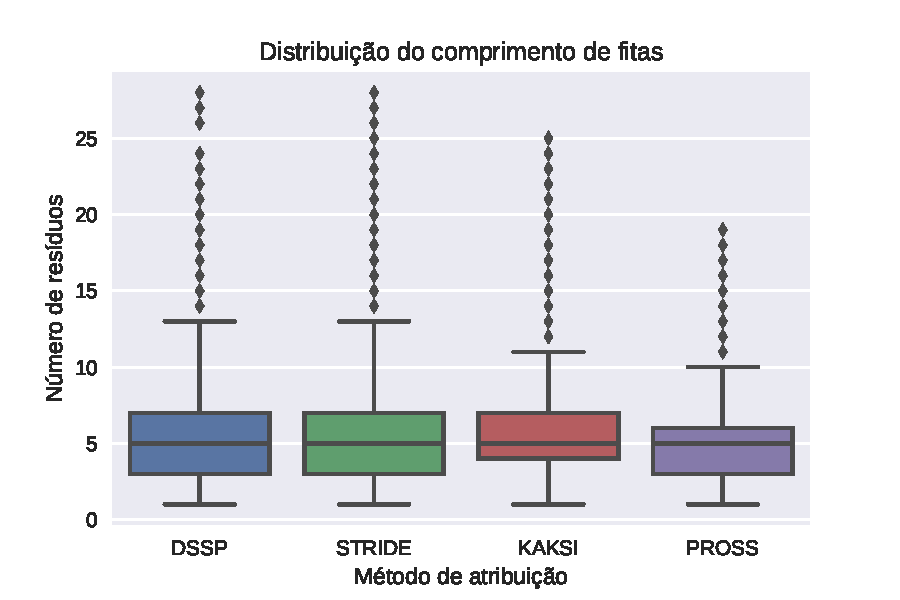
\includegraphics[width=\linewidth]{../figures/distribuicao_comprimento_fitas.pdf}
  \caption{Distribuição do comprimento de fitas por método de atribuição de estrutura secundária.}
  \label{fig:distribuicao_comprimento_fitas}
\end{figure}